\section{Design}
\begin{figure}
  \centering
  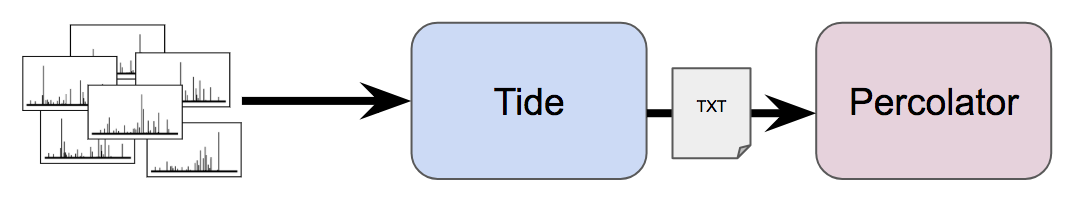
\includegraphics[scale=0.3]{serial_pipeline}
  \caption{Serial Pipeline}
  \label{fig:serial_pipeline}
\end{figure}
\begin{figure}
  \centering
  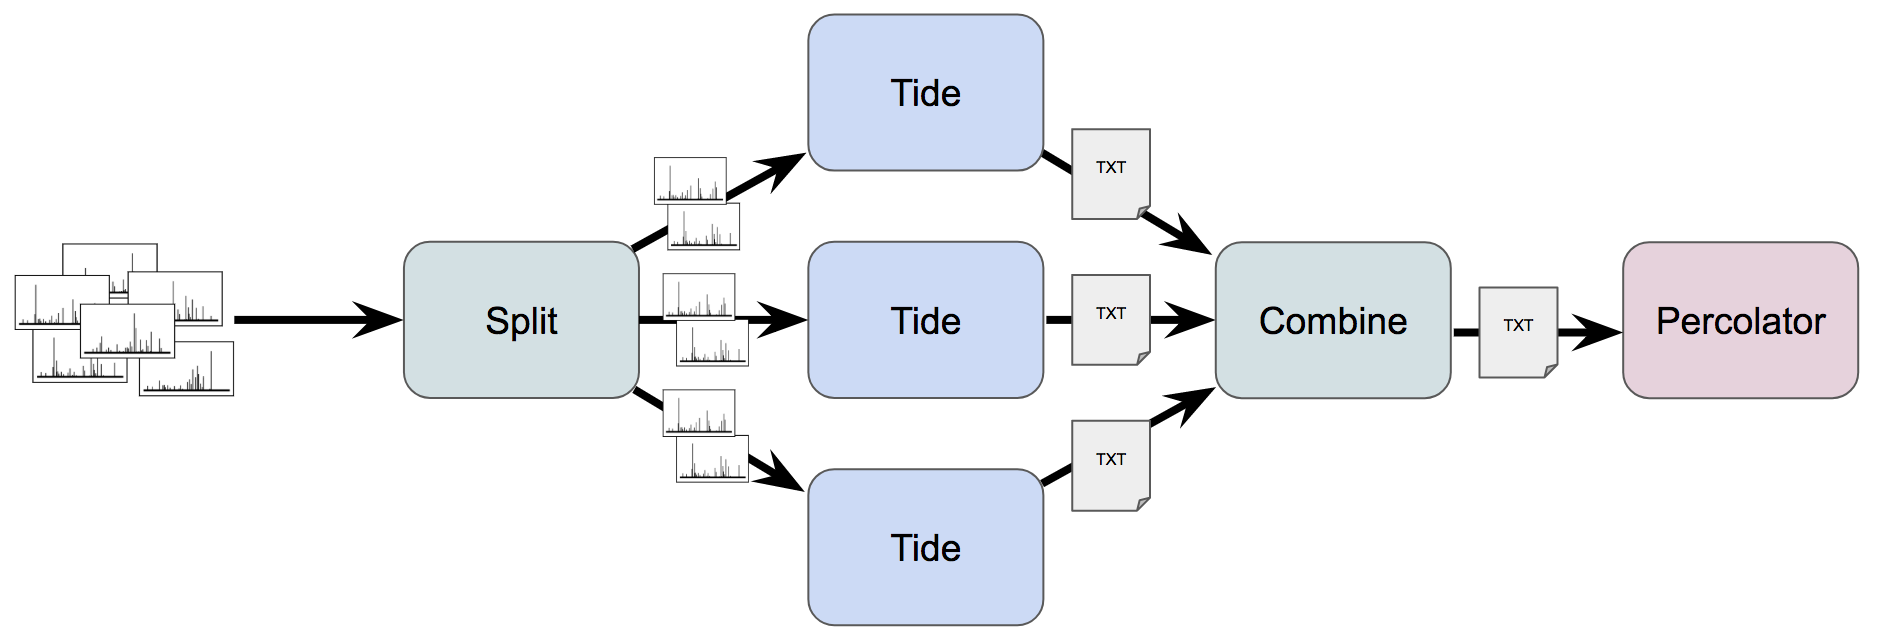
\includegraphics[scale=0.2]{lambda_pipeline}
  \caption{Lambda Pipeline}
  \label{fig:lambda_pipeline}
\end{figure}

The first attempt at designing \name tried to keep the pipeline as serial as possible, like in Figure \ref{fig:serial_pipeline}.
Initially, we used Comet, which is one of the most popular tools to analyze spectra\cite{comet}.
However, Comet was too slow and analyzing just one spectrum took Comet around five minutes in Lambda.
Since Lambda limits task execution time to five minutes, using Comet was not an ideal choice, as analyzing just one spectrum had a high chance of timing out.\\
\newline
Like Comet, Tide analyzes experimental spectra.
Tide creates FASTA database indices which decreases finding potential theoretical spectra matches by 79.5\% to 97.2\%\cite{crux}.
As shown in Figure \ref{fig:serial_pipeline}, in the serial pipeline, experimental spectra is given to Tide.
Tide processes the spectra and outputs the matches and these matches can be passed to Percolator.\\
\newline
Spectra files can be up to 3GB. Lambda provides 512MB of disk space and up to 3GB of memory, so processing an entire spectra file in one Lambda instance is not realistic.
To handle this problem, we split the input file into chunks,analyze each of these chunks on Tide in parallel.
The files outputted by Tide are significantly smaller and can fit in disk, so we are able to concat the resulting output files in a single Lambda instance.
Figure \ref{fig:lambda_pipeline} shows what the pipeline looks like on Lambda.
\newline

%\\Matching the experimental spectra against theoretical spectra can be extremely slow. To speed up the process, Tide can compute index values for the theoretical spectra and use these indices to speed up the search process.\\

